\subsection{Application: Aerospace Structural Health Monitoring and Turbofan Prognostics}

Aerospace structural health monitoring and propulsion prognostics are safety-critical machine-learning applications because prediction errors can directly affect maintenance planning, mission availability, operating cost, and safety margins. The objective is not merely to classify an asset as healthy or unhealthy. A useful prognostics system must infer degradation state, detect anomalous trajectories, estimate remaining useful life (RUL), and express uncertainty early enough for maintenance decisions to be scheduled before a fault becomes operationally critical.

Turbofan-engine prognostics is also a useful example of why benchmark protocol matters as much as model architecture. Remaining-life targets depend on the precise run-to-failure trajectory, and commonly used capped-RUL targets alter the learning problem relative to uncapped targets. Sensor selection, normalization, sliding-window construction, operating-condition handling, and engine-level train/test partitioning can all change reported RMSE and PHM scores. Results are therefore comparable only when these details match.

The NASA C-MAPSS benchmark provides a reproducible foundation for studying these issues. Its four standard subsets vary the number of operating conditions and fault modes, making it possible to distinguish performance on a relatively simple single-condition, single-fault setting from robustness under multiple operating regimes and multiple degradation mechanisms. The application below uses that benchmark structure to connect the chapter's optimization and validation principles to a realistic reliability-engineering workflow.

\textbf{Problem}

The engineering task is to estimate remaining useful life for each engine trajectory while minimizing both average prediction error and operationally dangerous late predictions. A model that achieves a low RMSE but systematically overestimates RUL near failure can be unacceptable because it delays maintenance exactly when the asset is approaching an unsafe regime.

\textbf{Dataset}

The application is organized around the NASA C-MAPSS turbofan degradation benchmark described in Pass20 [35]. The benchmark consists of multivariate run-to-failure trajectories divided into four commonly used subsets, FD001 through FD004. FD001 contains one operating condition and one fault mode; FD002 introduces multiple operating conditions; FD003 introduces multiple fault modes; and FD004 combines multiple operating conditions with multiple fault modes. Engine-level partitioning must be preserved so that windows from the same engine do not leak across training and evaluation splits.

\textbf{Model}

A typical RUL model consumes a sliding window of sensor and operating-condition measurements and maps that window to a scalar remaining-life estimate. Classical baselines include linear regression, support-vector regression, and random forests. Sequence models include LSTMs and GRUs, convolutional models treat the sensor-by-time window as a structured signal, and attention or transformer architectures model longer-range temporal interactions. The model family is less important than maintaining a matched preprocessing and target-construction protocol when comparing methods.

\textbf{Method}

Let \(x_{e,t}\in\mathbb{R}^{p}\) denote the sensor and operating-condition vector for engine \(e\) at cycle \(t\). For a window length \(L\), the model receives \(X_{e,t}=[x_{e,t-L+1},\ldots,x_{e,t}]\) and predicts \(\hat r_{e,t}=f_\theta(X_{e,t})\). For a training engine that fails at cycle \(T_e\), the uncapped target is \(r_{e,t}=T_e-t\). When a capped target is used, the cap value must be reported because it changes both the early-life target distribution and the resulting error profile. Optimization settings, window length, stride, sensor subset, normalization rule, early stopping, and random seeds are all recorded as part of the reproducibility protocol.

\textbf{Evaluation}

Evaluation combines symmetric regression metrics with the asymmetric PHM score. RMSE and MAE summarize average numerical error, while the PHM score penalizes late RUL predictions more severely than early predictions of the same magnitude. Listing~\ref{lst:ch1-phm-score} makes that asymmetry explicit: line 5 computes signed RUL error, lines 6--7 apply different exponential penalties to early and late predictions, and line 8 aggregates the per-engine penalties. The code makes clear why two models with similar RMSE can receive very different prognostic scores when one model systematically overestimates remaining life near failure.

\begin{lstlisting}[style=BookCode,language=Python,caption={Asymmetric PHM08 prognostic scoring function.},label={lst:ch1-phm-score}]
def phm_score(y_true_rul, y_pred_rul):
    y_true = np.asarray(y_true_rul, dtype=float)
    y_pred = np.asarray(y_pred_rul, dtype=float)
    if y_true.shape != y_pred.shape:
        raise ValueError("shape mismatch")
    error = y_pred - y_true
    scores = np.where(error < 0,
                      np.exp(-error / 13.0) - 1.0,
                      np.exp(error / 10.0) - 1.0)
    return float(np.sum(scores))
\end{lstlisting}

Figure~\ref{fig:ch1-turbofan-prognostics} provides a reproducible numerical prognostics rendering: panel (a) shows multiple degradation trajectories with engine-specific degradation rates, and panel (b) shows a reference remaining-life trajectory together with a noisy model estimate. The figure is deliberately identified as a numerical reconstruction rather than as a plot of NASA records.

\begin{figure}[t]
\centering
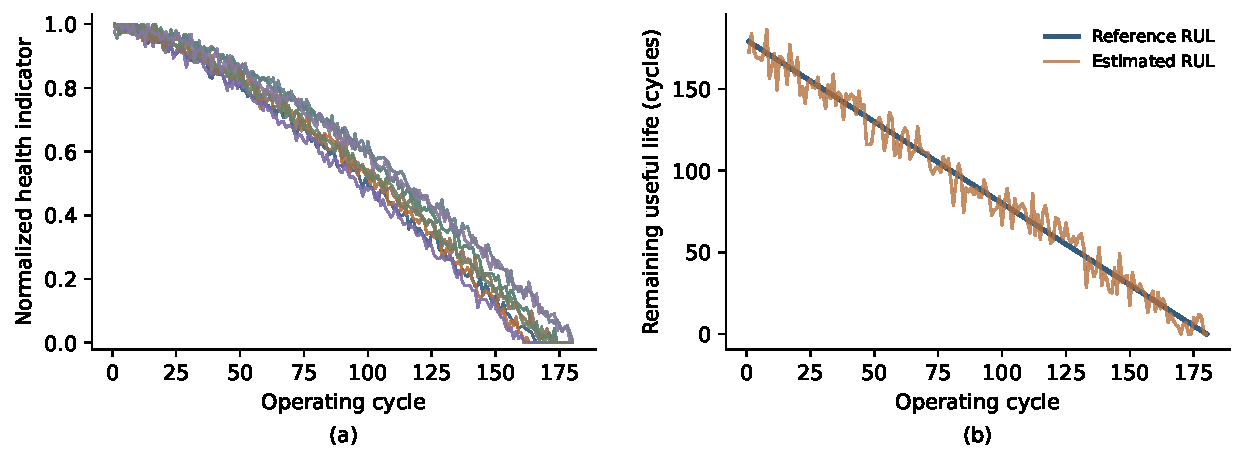
\includegraphics[width=\BookFigureWidth]{figures/ch01_turbofan_prognostics.pdf}
\caption{Numerical turbofan-prognostics rendering used to illustrate trajectory-level degradation and remaining-useful-life estimation without misrepresenting simulated curves as NASA C-MAPSS measurements. (a) Eight engine-like normalized health trajectories with different degradation rates and small stochastic perturbations. (b) Reference remaining useful life for one trajectory and a noisy estimated RUL sequence. The numerical reconstruction is used only to illustrate evaluation structure; empirical benchmark claims are taken from the cited C-MAPSS literature and must be compared under matched preprocessing and scoring conventions.}
\label{fig:ch1-turbofan-prognostics}
\end{figure}

\begin{table}[t]
\centering
\small
\caption{Published C-MAPSS benchmark anchors retained from the Pass20 evidence review. The values are not directly interchangeable across papers unless the RUL cap, sensor subset, normalization, windowing, train/test files, and scoring convention match.}
\label{tab:ch1-cmapss-benchmark}
\begin{tabular}{lll}
\toprule
Method or study anchor & Dataset & Reported metric \\
\midrule
LSTM sequence model & FD001 / FD003 & RMSE 16.14 / 16.18; score 338 / 852 \\
Ensemble recurrent model & FD001 / FD003 & RMSE 14.57 / 14.92 \\
BiLSTM autoencoder & FD001 & RMSE 14.70; score 273.00 \\
Attention-LSTM & FD001 & RMSE 14.53; score 322.44 \\
CNN+FNN PHM comparison & FD001--FD004 & scores 1287 / 13,570 / 1596 / 7886 \\
\bottomrule
\end{tabular}
\end{table}

\textbf{Results}

The published anchors demonstrate why a single FD001 number is insufficient for judging a prognostics method. Recurrent, convolutional, attention-based, and ensemble models can all produce competitive FD001 error, yet performance can change materially on FD002--FD004 when operating conditions and fault modes vary. For this reason, Table~\ref{tab:ch1-cmapss-benchmark} is used as a protocol-aware comparison rather than a leaderboard.

\textbf{Error Analysis}

Error analysis is performed by engine trajectory, benchmark subset, operating regime, and degradation stage. Early-life predictions are often nearly constant when capped-RUL targets are used, while late-life prediction requires the model to detect accelerating degradation. Residuals should therefore be stratified into early, middle, and late life, with particular attention to positive RUL error near failure because late predictions are penalized more severely by the PHM score. Additional diagnostics should identify whether specific sensor channels or operating conditions dominate the error.

\textbf{Limitations}

The figure in this Application is a reproducible numerical rendering, not a substitute for a protocol-matched C-MAPSS experiment. The benchmark values in Table~\ref{tab:ch1-cmapss-benchmark} come from published studies summarized in Pass20 and should not be recombined as though all studies used identical preprocessing. A final reproduced benchmark requires the exact NASA files, an explicit RUL-cap policy, the selected sensors, the normalization procedure, the train/test protocol, and the scoring implementation.

\textbf{Deployment / Engineering Implications}

Aerospace prognostics is a reliability-engineering workflow rather than an isolated regression benchmark. Deployed systems must preserve trajectory provenance, monitor sensor drift, quantify prediction uncertainty, detect changes in operating regime, and connect RUL estimates to maintenance scheduling rules. A model that improves average RMSE but produces hazardous late predictions near failure should not be promoted solely on the basis of the aggregate error metric.
